\documentclass[12pt,a4paper]{amsart}

\usepackage[T1]{fontenc}
\usepackage[utf8]{inputenc}
\usepackage[british]{babel}
\usepackage{mathtools}
\usepackage{amsthm}
\usepackage{amssymb}
\usepackage{mathrsfs}
\usepackage{enumitem}
\usepackage{tikz-cd}
\usetikzlibrary{decorations.markings}
\usepackage{float}
\usepackage{hyperref}
\urlstyle{same}
\usepackage[noabbrev]{cleveref}

\theoremstyle{plain}
\newtheorem{thm}{Theorem}[section]
\newtheorem*{thm*}{Theorem}
\newtheorem{lm}[thm]{Lemma}
\newtheorem{prop}[thm]{Proposition}
\newtheorem{cor}[thm]{Corollary}
\theoremstyle{definition}
\newtheorem{defn}[thm]{Definition}
\newtheorem{exmp}[thm]{Example}
\newtheorem{xca}[thm]{Exercise}
\theoremstyle{remark}
\newtheorem{rem}[thm]{Remark}
\Crefname{thm}{Theorem}{Theorems}
\Crefname{lm}{Lemma}{Lemmas}
\Crefname{prop}{Proposition}{Propositions}
\Crefname{cor}{Corollary}{Corollaries}
\Crefname{defn}{Definition}{Definitions}
\Crefname{exmp}{Example}{Examples}
\Crefname{xca}{Exercise}{Exercises}
\Crefname{rem}{Remark}{Remarks}

\title[Hilbert schemes of points on surfaces]{Hilbert schemes of points on surfaces}
\author[Pedro N\'{u}\~{n}ez]{Pedro N\'{u}\~{n}ez}
\address{Pedro N\'{u}\~{n}ez \newline
\indent Albert-Ludwigs-Universit\"{a}t Freiburg, Mathematisches Institut \newline
\indent Ernst-Zermelo-Straße 1, 79104 Freiburg im Breisgau (Germany)}
\email{\normalfont\href{mailto:pedro.nunez@math.uni-freiburg.de}{pedro.nunez@math.uni-freiburg.de}}
\renewcommand*{\urladdrname}{\itshape Homepage}
\urladdr{\normalfont\href{https://home.mathematik.uni-freiburg.de/nunez/}{https://home.mathematik.uni-freiburg.de/nunez}}
\thanks{The author gratefully acknowledges support by the DFG-Graduiertenkolleg GK1821 ``Cohomological Methods in Geometry'' at the University of Freiburg.}
\date{8th June 2021}

\setcounter{tocdepth}{1}
\sloppy
\makeatletter
\hypersetup{
  pdfauthor={\authors},
  pdftitle={\@title},
  colorlinks,
  linkcolor=[rgb]{0.2,0.2,0.6},
  citecolor=[rgb]{0.2,0.6,0.2},
  urlcolor=[rgb]{0.6,0.2,0.2}}
\makeatother

\begin{document}

\maketitle

\begin{abstract}
  Script for the seventh talk of the seminar on Heisenberg algebras and Hilbert schemes of points on surfaces organized by Mara Ungureanu during the Summer Term 2021 at the University of Freiburg.
\end{abstract}

\tableofcontents

\setcounter{section}{-1}

\section{Conventions and notation}

We always work over $\mathbb{C}$.
By a variety we mean an integral separated scheme of finite type over $\mathbb{C}$ as in \cite{har77}.
Similarly, curves and surfaces are always implicitly assumed to be irreducible.
The main reference for the talk is \cite[\S 1]{nak99}.

Let $n > 0$ be a natural number and let $X$ be a quasi-projective scheme.
Then we denote by $\mathfrak{S}_{n}$ the symmetric group of order $n$, by $X^{\times n}$ the $n$-fold product of $X$ with itself and by $X^{[n]}$ the Hilbert scheme of $n$-points on $X$.

Let us fix the natural number $n > 0$ from now on.

\section{Introduction}

We would like to parametrize unordered tuples of $n$-points on a smooth projective surface $X$.
A natural candidate for parameter space would be the quotient $S^{n}X$ of the product $X^{\times n}$ by the $\mathfrak{S}_{n}$-action permuting the factors.
But $S^{n}X$ has singularities, so instead we look at the Hilbert scheme of points $X^{[n]}$.
We will see that there is a morphism $\pi \colon X^{[n]} \to S^{n}X$, called the \textit{Hilbert--Chow} morphism, which is a resolution of singularities.

\section{Symmetric products and their stratification}

\begin{defn}[Symmetric products]
  Let $X$ be a quasi-projective variety.
  We define the \textit{$n$-th symmetric product of $X$}, denoted $S^{n}X$, to be the quotient of $X^{\times n}$ by the action of $\mathfrak{S}_{n}$ which permutes the factors.
\end{defn}

\begin{rem}
  Quotients of quasi-projective varieties by algebraic actions of finite groups are discussed in \Cref{sec:quotient}.
  It is shown in \Cref{thm:quotient} that the quotient $S^{n}X$ exists as a scheme and is in fact a quasi-projective variety.
  The fibers of the quotient morphism over closed points are precisely the orbits of closed points in $X$, and the quotient space carries the quotient topology induced by the quotient morphism.
  Moreover, let $\mathbf{P}$ be any of the following properties:
  \begin{itemize}
    \item affine,
    \item projective,
    \item normal.
  \end{itemize}
  If $X$ is $\mathbf{P}$, then $S^{n}X$ is $\mathbf{P}$.
  In particular, $S^{n}X$ is a normal projective variety if $X$ was a smooth projective variety.
\end{rem}

\begin{exmp}\label{exmp:affineline}
  $S^{n}(\mathbb{A}^{1}) \cong \mathbb{A}^{n}$.
  
  \begin{proof}
    Indeed, it follows from \Cref{cor:affinequotient} that
    \[ S^{n}(\mathbb{A}^{1}) = \operatorname{Spec}\left(\mathbb{C}[x_{1}, \ldots, x_{n}]^{\mathfrak{S}_{n}}\right), \]
    so the claim follows from the \href{https://en.wikipedia.org/wiki/Elementary_symmetric_polynomial#Fundamental_theorem_of_symmetric_polynomials}{fundamental theorem of symmetric polynomials}.
  \end{proof}
\end{exmp}

In order to show later that the yet-to-be-defined Hilbert--Chow morphism $\pi \colon X^{[n]} \to S^{n}X$ is a resolution of singularities in the case of surfaces, it will be convenient to consider the following stratification of $S^{n}X$.

Let $k \in \mathbb{N}_{>0}$ such that $k \leq n$.
Consider a tuple $\nu = (\nu_{1}, \ldots, \nu_{k})$ with $\nu_{1} \geq \nu_{2} \geq \ldots \geq \nu_{k} > 0$ such that $n = \nu_{1} + \ldots + \nu_{k}$.
Call this a \textit{partition of $n$} of \textit{length} $l(\nu) := k$.
Then, for each partition $\nu$ of $n$, we define
\[ S^{n}_{\nu}X := \left\{ \quad \sum_{i = 1}^{l(\nu)} \nu_{i}[x_{i}] \in S^{n}X \quad \middle| \quad x_{i} \neq x_{j} \text{ for } i \neq j \quad \right\}. \]

\begin{lm}\label{lm:stratification}
  Denote by $P(n)$ the set of partitions of $n$ as defined above and let $X$ be a quasi-projective variety.
  Then:
  \begin{enumerate}[label=(\roman*)]
    \item The collection $\{ S_{\nu}^{n}X \}_{\nu \in P(n)}$ is a stratification of $S^{n}X$.
    \item For all $\nu \in P(n)$ we have $\dim(S_{\nu}^{n}X) = l(\nu)\dim(X)$.
    \item The stratum $S_{(1,\ldots,1)}^{n}X$ is open.
  \end{enumerate} 
  \begin{proof}
    Let $\nu \in P(n)$ be a partition of length $k$.
    We have only defined $S^{n}_{\nu}X$ as a subset of closed points in $S^{n}X$, so let us first check that it is in fact an irreducible and locally closed subset of the set of closed points in $S^{n}X$.
    By definition there are natural numbers $\nu_{1} \geq \nu_{2} \geq \ldots \geq \nu_{k} > 0$ such that $n = \nu_{1} + \ldots + \nu_{k}$ and $\nu = (\nu_{1},\ldots, \nu_{k})$.
    Consider the $\mathbb{C}$-scheme morphism
    \begin{align*}
      f \colon X^{\times k} & \longrightarrow X^{\times n} \\
      (x_{1}, \ldots, x_{k}) & \longmapsto (x_{1}, \ldots, x_{1}, \ldots, x_{k}, \ldots, x_{k})
    \end{align*}
    in which $x_{i}$ appears $\nu_{i}$ times on the right hand side for each $i \in \{1, \ldots, k \}$.
    We may then compose this with the quotient morphism $q \colon X^{\times n} \to S^{n}X$ to obtain a $\mathbb{C}$-scheme morphism $h \colon X^{\times k} \to S^{n}X$.
    Let $U \subseteq X^{\times k}$ be the dense open subset of tuples $(x_{1}, \ldots, x_{k})$ such that $x_{i} \neq x_{j}$ whenever $i \neq j$.
    Then we have $S^{n}_{\nu}X = h(U)$, and this is what we want to show to be an irreducible locally closed subset.
    Irreducibility follows from $U$ being irreducible, which in turn follows from $U$ being a dense open subset of the irreducible space $X^{\times k}$.
    To show that it is locally closed, we note first that $f(X^{\times k})$ is a closed subset in $X^{\times n}$.
    And the quotient morphism $q$ is finite, in particular closed, so $h(X^{\times k})$ is also a closed subset of $S^{n}X$.
    Next we look at the dense open subset $V \subseteq X^{\times n}$ of $n$-tuples of points in which there are at least $k$ distinct points, so that $f(U) = V \cap f(X^{\times k})$.
    This is a $\mathfrak{S}_{n}$-invariant open subset, which in turn has two implications that we are interested in.
    First, $q(V)$ is open, because $q^{-1}(q(V)) = V$ and $S^{n}X$ carries the quotient topology induced by $q$.
    Second, $q(V \cap Z) = q(V) \cap q(Z)$ for all $Z \subseteq X^{\times n}$, because if $q(v) = q(z)$ for $v \in V$ and $z \in Z$, then $z \in V$ as well.
    Therefore we can write
    \begin{align*}
      S_{\nu}^{n}X & = h(U) \\
      & = q(f(U)) \\
      & = q(V \cap f(X^{\times k})) \\
      & = q(V) \cap q(f(X^{\times k})) \\
      & = q(V) \cap h(X^{\times k}),
    \end{align*}
    expressing $S_{\nu}^{n}X$ as an interseciton of the open subset $q(V)$ and the closed subset $h(X^{\times k})$.
    This proves that $S_{\nu}^{n}X$ is a locally closed subset of $S^{n}X$.
    Moreover, it also shows that $\dim(S_{\nu}^{n}X) = l(\nu)\dim(X)$, because $h$ has finite fibers over closed points.
    So we get $(ii)$.
    If $k = n$, i.e.~if $S^{n}_{\nu}X = S^{n}_{(1,\ldots, 1)}X$, then $f = \operatorname{id}_{X^{\times n}}$ and $U$ is the $\mathfrak{S}_{n}$-invariant dense open subset of $X^{\times n}$ consisting of tuples without any repetitions.
    Since it is $\mathfrak{S}_{n}$-invariant, $q(U) = h(U)$ is a dense open subset as well, which proves $(iii)$.
    
    Now we check that these irreducible, locally closed subsets form a stratification of $S^{n}X$.
    As sets, looking only at the closed points as usual, we can write
    \[ S^{n}X = \bigsqcup_{\nu \in P(n)} S^{n}_{\nu}X. \]
    It remains to show that if $S^{n}_{\nu'}X$ intersects the closure of $S^{n}_{\nu}X$ in $S^{n}X$, then $S^{n}_{\nu'}X$ is contained in this closure.
    First we compute the closure of $S^{n}_{\nu}X$ in $S^{n}X$.
    The claim is that
    \[ \overline{S^{n}_{\nu}X} = \left\{ \sum_{i=1}^{k} \nu_{i} [x_{i}] \in S^{n}X \right\}, \]
    where $k = l(\nu)$.
    So we may have more repetitions than the ones originally prescribed by the partition $\nu$.
    Since $q$ is surjective, closed and continuous, we have
    \[ \overline{S^{n}_{\nu}X} = q(\overline{q^{-1}(S^{n}_{\nu}X)}). \]
    The preimage $q^{-1}(S^{n}_{\nu}X)$ consists of tuples $(x_{1}, \ldots, x_{n})$ in which there are exactly as many repetitions as prescribed by $\nu$, meaning that for each $i \in \{1, \ldots, k\}$ there exists some $x_{i} \in X$ such that $x_{i}$ appears exactly $\nu_{i}$ times in $(x_{1}, \ldots, x_{n})$.
    The analytic topology is finer than the Zariski topology, so the Zariski closure of $q^{-1}(S^{n}_{\nu}X)$ contains the closure of $q^{-1}(S^{n}_{\nu}X)$ in the analytic topology.
    The closure in the analytic topology can be computed using limits of sequences, and we see that it consists of tuples $(x_{1}, \ldots, x_{n})$ in which there are at least as many repetitions as prescribed by $\nu$, i.e.~meaning precisely that after taking the quotient by the $\mathfrak{S}_{n}$-action we do get the claimed description.
    So we would like to check that this is also the Zariski closure, for which it suffices to show that this is a Zariski closed subset.
    This set is cut out by requiring a finite list of equalities between pairs of coordinates in the tuples of $X^{\times n}$, hence it is indeed Zariski closed.
    This proves that the closure is described as we claimed above.
    Now if $\sum_{i=1}^{l(\nu')}\nu_{i}'[x_{i}]$ is an element in $S^{n}_{\nu'}X$ which belongs also to $\overline{S^{n}_{\nu}X}$, then $\nu'$ prescribes at least as many repetitions as $\nu$ does in the sense made precise earlier.
    Therefore $S^{n}_{\nu'}X \subseteq \overline{S^{n}_{\nu}X}$, which is what we needed to show and concludes the proof of $(i)$.
  \end{proof}
\end{lm}

\begin{lm}\label{lm:smoothstratum}
  In the situation of \Cref{lm:stratification}, if we assume moreover that $X$ is smooth, then $S^{n}_{(1, \ldots, 1)}X$ is smooth as well.
  
  \begin{proof}
    Let $U \subseteq X^{\times n}$ denote the dense and $\mathfrak{S}_{n}$-invariant open subset of tuples without any repetitions.
    Then the finite group $\mathfrak{S}_{n}$ acts freely on $U$.
    This implies that the quotient morphism $q$ is locally free over $S^{n}_{(1,\ldots,1)}X$, see Theorem (4.16) in \url{https://www.math.ru.nl/~bmoonen/BookAV/Quotients.pdf}.
    Since each fiber over $S^{n}_{(1, \ldots, 1)}X$ consists of exactly $\deg(q)$ points, $q$ is also unramified over $S^{n}_{(1, \ldots, 1)}X$.
    Flat and unramified implies étale \cite[Exercise III.10.3]{har77}, so the morphism $q$ is also smooth over $S^{n}_{(1, \ldots, 1)}X$.
    We may now apply \cite[\href{https://stacks.math.columbia.edu/tag/02K5}{Tag 02K5}]{stacks-project} to conclude that $S^{n}_{(1, \ldots, 1)}X \to \operatorname{Spec}(\mathbb{C})$ is smooth as well, i.e.~$S^{n}_{(1, \ldots, 1)}X$ is smooth.

    One could also argue analytic locally using the fact that free actions of finite groups on Hausdorff spaces are properly discontinuous, cf.~\cite[Exercise III.7.1]{bre97}.
  \end{proof}
\end{lm}

\begin{exmp}
  Let us look at the case of $X = \mathbb{A}^{2}$ and $n = 2$.
  We want to study the singularities of $S^{2}\mathbb{A}^{2}$.
  By \Cref{lm:smoothstratum} we only need to study the points outside of $S^{2}_{(1,1)}\mathbb{A}^{2}$.
  Consider for example the point $2[(0,0)]$.
  We know that $S^{2}\mathbb{A}^{2}$ has dimension $4$, because it is the quotient of the $4$-dimensional variety $\mathbb{A}^{2} \times \mathbb{A}^{2}$ by the action of a finite group.
  More precisely, if we identify $(\mathbb{A}^{2})^{\times 2}$ with $\mathbb{A}^{4}$ and $\mathfrak{S}_{2}$ with $\mathbb{Z}/2\mathbb{Z}$, the action of $1 + 2\mathbb{Z} \in \mathbb{Z}/2\mathbb{Z}$ on the coordinate ring $A := \mathbb{C}[x_{1}, y_{1}, x_{2}, y_{2}]$ is given by the $\mathbb{C}$-algebra homomorphism uniquely determined by
  \begin{align*}
    x_{1} & \mapsto x_{2}, \\
    y_{1} & \mapsto y_{2}, \\
    x_{2} & \mapsto x_{1}, \\
    y_{2} & \mapsto y_{1}.
  \end{align*}
  The coordinate ring of $S^{2}\mathbb{A}^{2}$ is then the subring of $\mathbb{Z}/2\mathbb{Z}$-invariants.
  For example, the following polynomials are invariant under this action:
  \begin{align*}
    x_{1} + x_{2}, \\
    y_{1} + y_{2}, \\
    x_{1}x_{2}, \\
    y_{1}y_{2}.
  \end{align*}
  These all belong to the ideal $\mathfrak{m}$ of the point $2[(0,0)]$, because this point is the image of $(0,0,0,0) \in \mathbb{A}^{4}$ and the quotient morphism is obtained by intersecting each prime ideal with the subring of $\mathbb{Z}/2\mathbb{Z}$-invariants.
  But the polynomial $x_{1}y_{1} + x_{2}y_{2}$ is also in $\mathfrak{m}$, and we claim that these $5$ polynomials are $\kappa(\mathfrak{m})$-linearly independent in $\mathfrak{m}/\mathfrak{m}^{2}$.
  Since $\mathfrak{m}$ is maximal, we can write $\kappa(\mathfrak{m}) = (A^{\mathbb{Z}/2\mathbb{Z}})/\mathfrak{m}$.
  So suppose we have polynomials $f_{1}, \ldots, f_{4} \in A^{\mathbb{Z}/2\mathbb{Z}}$ such that there exists some polynomial $g \in \mathfrak{m}^{2}$ such that
  \[ x_{1}y_{1} + x_{2}y_{2} + f_{1}(x_{1} + x_{2}) + f_{2}(y_{1} + y_{2}) + f_{3}x_{1}x_{2} + f_{4}y_{1}y_{2} = g. \]
  Since polynomials in $\mathfrak{m}$ have zero constant term, any non-zero monomial appearing as a term of $g$ has total degree at least $2$.
  We claim first that the total degree $2$ part of $g$ has to be zero.
  Indeed, we can argue by contradiction looking at the total degree $2$ part of the previous equation.
  The only homogeneous polynomials of total degree $1$ in $\mathfrak{m}$ are the $\mathbb{C}$-linear combinations of $x_{1} + x_{2}$ and $y_{1} + y_{2}$.
  So assuming that the total degree $2$ part of $g$ is zero, we may write the total degree $2$ part of the previous equation as
  \begin{align*}
    x_{1}y_{1} + x_{2}y_{2} + (\lambda_{1}x_{1} + \mu_{1}y_{1} + \lambda_{1} x_{2} + \mu_{1} y_{2})(x_{1} + x_{2}) \\
    + (\lambda_{2} x_{1} + \mu_{2} y_{1} + \lambda_{2} x_{2} + \mu_{2} y_{2})(y_{1} + y_{2}) + \lambda x_{1}x_{2} + \mu y_{1} y_{2} = 0 
  \end{align*}
  for some $\lambda, \mu, \lambda_{1}, \lambda_{2}, \mu_{1}, \mu_{2} \in \mathbb{C}$.
  Writing out the product we see that the coefficient of $x_{1}^{2}$ is $\lambda_{1}$, which must therefore be zero.
  And similarly, the coefficient of $y_{1}^{2}$ is $\mu_{2}$, which must then be zero.
  Grouping coefficients we obtain the system of equations
  \[
    \begin{cases}
      \lambda = 0 \\
      \mu = 0 \\
      \mu_{1} + \lambda_{2} = 0 \\
      1 + \mu_{1} + \lambda_{2} = 0
    \end{cases}
  \]
  The system does not have any solution, so we reach the desired contradiction.
  Therefore $g$ must have a non-zero homogeneous total degree $2$ part.
  As explained above, this has to be the product of two $\mathbb{C}$-linear combinations of $x_{1} + x_{2}$ and $y_{1} + y_{2}$, say, the product of $\alpha_{1}(x_{1} + x_{2}) + \beta_{1}(y_{1} + y_{2})$ and $\alpha_{2}(x_{1} + x_{2}) + \beta_{2}(y_{1} + y_{2})$ with $\alpha_{1}, \beta_{1}, \alpha_{2}, \beta_{2} \in \mathbb{C}$.
  With the same notation as above for the left hand side of the equation we would obtain the system of equations
  \[
    \begin{cases}
      1 + \mu_{1} + \lambda_{2} - \alpha_{1} \beta_{2} - \alpha_{2} \beta_{1} = 0 \\
      \lambda_{1} - \alpha_{1} \alpha_{2} = 0 \\
      \lambda + 2 \lambda_{1} - 2 \alpha_{1} \alpha_{2} = 0 \\
      \mu_{2} - \beta_{1} \beta_{2} =  0 \\
      \mu + 2 \mu_{2} - 2 \beta_{1} \beta_{2} = 0 \\
      \mu_{1} + \lambda_{2} - \alpha_{1} \beta_{2} - \alpha_{2} \beta_{1} = 0
    \end{cases}
  \]
  The system still does not have any solution, so we have a contradiction in any case.
  Therefore the $5$ polynomials are $\kappa(\mathfrak{m})$-linearly independent in $\mathfrak{m}/\mathfrak{m}^{2}$, which shows that $2[(0,0)]$ is a singular point in $S^{2}\mathbb{A}^{2}$.

  More generally, the same arguments show that $S^{n}\mathbb{A}^{2}$ is singular at $n[(0,\ldots,0)]$ for any $n \geq 2$, cf.~\cite[Example 3.5]{rot16}.
  But for $n = 2$ we can still say a bit more about the geometry of the singularities, so let us do that following \cite[Example 3.6]{rot16}.
  We consider the basis $(1, 0, 1, 0)$, $(0, 1, 0, 1)$, $(1, 0, -1, 0)$ and $(0, 1, 0, -1)$ on $\mathbb{A}^{4}$, so that the action of $\mathbb{Z}/2\mathbb{Z}$ on the new coordinate ring $R = \mathbb{C}[x, y, u, v]$ is given by
  \begin{align*}
    x \mapsto x, \\
    y \mapsto y, \\
    u \mapsto -u, \\
    v \mapsto -v.
  \end{align*}
  We can think now of this action on $\mathbb{A}^{4} \cong \mathbb{A}^{2} \times \mathbb{A}^{2}$ as acting only on the second factor, which is the one corresponding to the coordinates $u$ and $v$.
  We check first what the quotient is in this case.
  A $\mathbb{Z}/2\mathbb{Z}$-invariant polynomial in $\mathbb{C}[u,v]$ can have only monomials of even total degree.
  Indeed, the monomials $u^{2}$, $uv$ and $v^{2}$ are all in $\mathbb{C}[u,v]^{\mathbb{Z}/2\mathbb{Z}}$, so all the monomials of even total degree are in this subalgebra as well, i.e.~$\mathbb{C}[u^{2}, uv, v^{2}] \subseteq \mathbb{C}[u,v]^{\mathbb{Z}/2\mathbb{Z}}$.
  If $f(u,v)$ is a $\mathbb{Z}/2\mathbb{Z}$-invariant polynomial, we may substract from it all its even total degree monomials.
  The result will be a $\mathbb{Z}/2\mathbb{Z}$-invariant polynomial $h$ with the property that $h(-u,-v) = -h(u,v)$ for all $(u, v) \in \mathbb{A}^{2}$.
  It follows from $\mathbb{Z}/2\mathbb{Z}$-invariance that we must have $h(u,v) = 0$ for all $(u, v) \in \mathbb{A}^{2}$, hence $h = 0$ and $f \in \mathbb{C}[u^{2},uv,v^{2}]$.
  This shows that the coordinate ring of the quotient of $\mathbb{A}^{2}$ by this $\mathbb{Z}/2\mathbb{Z}$-action is $\mathbb{C}[u^{2}, uv, v^{2}]$.
  We have a surjective $\mathbb{C}$-algebra homomorphism
  \begin{align*}
    \phi \colon \mathbb{C}[a,b,c] & \longrightarrow \mathbb{C}[u^{2}, uv, v^{2}] \\
    a & \longmapsto u^{2}, \\
    b & \longmapsto uv, \\
    c & \longmapsto v^{2}.
  \end{align*}
  So we may rewrite the coordinate ring of the quotient as $\mathbb{C}[a,b,c]/\ker(\phi)$.
  We have $(b^{2} - ac) \subseteq \ker(\phi)$, so $V(\ker(\phi)) \subseteq V(b^{2} - ac)$ in $\mathbb{A}^{3}$.
  But both of them are irreducible closed subsets of $\mathbb{A}^{3}$ of the same dimension, so they must be equal.
  Since both $(b^{2} - ac)$ and $\ker(\phi)$ are prime ideals, this implies that they are equal.
  So the coordinate ring of the quotient is $\mathbb{C}[a,b,c]/(b^{2} - ac)$ and we see that the quotient is the cone over the smooth conic $\{ [a:b:c] \in \mathbb{P}^{2} \mid b^{2} - ac \}$ \cite[Exercise I.2.10]{har77}.
  
  Let us denote $G := \mathbb{Z}/2\mathbb{Z}$.
  Coming back to the $G$-action on $\mathbb{A}^{2} \times \mathbb{A}^{2}$, we consider the $G$-invariant morphism $\mathbb{A}^{2} \times \mathbb{A}^{2} \to \mathbb{A}^{2} \times (\mathbb{A}^{2}/G)$, which is given by the universal property of the product applied to the projection $p_{1} \colon \mathbb{A}^{2} \times \mathbb{A}^{2} \to \mathbb{A}^{2}$ and the composition of the projection $p_{2} \colon \mathbb{A}^{2} \times \mathbb{A}^{2} \to \mathbb{A}^{2}$ and the quotient $q_{2} \colon \mathbb{A}^{2} \to \mathbb{A}^{2}/G$, where this last quotient morphisms corresponds to the action that we were discussing earlier, i.e.~$\mathbb{A}^{2}/G$ is the cone over the conic above.
  This morphism is indeed $G$-invariant, because $G$ acts trivially on the first factor.
  So we obtain a $\mathbb{C}$-scheme morphism
  \[ \psi \colon \mathbb{A}^{4}/G \to \mathbb{A}^{2} \times (\mathbb{A}^{2}/G). \]
  We claim that it is an isomorphism.
  Indeed, it follows from the explicit description of closed points in the quotient by the action of a finite group that $\psi$ is bijective on closed points.
  Moreover, the right hand side is normal, because it is the product of two normal varieties, cf.~\url{https://mathoverflow.net/a/2058/99436}.
  This already implies that $\psi$ is an isomorphism; see \url{https://mathoverflow.net/a/264216} for a detailed argument combining various versions of Zariski's Main Theorem.

  Putting all the discussion above together, we see that the quotient of $\mathbb{A}^{4}$ by the $\mathbb{Z}/2\mathbb{Z}$-action is the product of the affine plane and the cone over a smooth conic, hence giving a more explicit description of the singularities of the quotient.
\end{exmp}

\section{Hilbert--Chow morphism}

\begin{prop}
  Let $X$ be a quasi-projective surface.
  Then the formula
  \begin{align*}
    \pi \colon X^{[n]} & \longrightarrow S^{n}X \\
    [Z] & \longmapsto \sum_{x \in X} \dim_{\mathbb{C}}(\mathscr{O}_{Z,x})[x] 
  \end{align*}
  defines a $\mathbb{C}$-scheme morphism called the \textit{Hilbert--Chow morphism}.
  
  \begin{proof}
    We sketch the construction of the corresponding morphism following \cite[\S 3.2]{leh00}.
    A similar but slightly different construction of the same morphism can be found in \cite[p.~41]{ber08}; the core of the argument seems to be essentially the same but the reduction steps are not exactly the same.
    The idea in any case is to define $\pi$ at the level of representable functors and then obtain the morphism at the level of varieties by Yoneda.
    Let $\mathcal{H}ilb^{n}_{X}$ be the functor represented by $X^{[n]}$ and let $h_{S^{n}X}$ be the functor represented by $S^{n}X$.
    We want a natural transformation $\eta \colon \mathcal{H}ilb^{n}_{X} \to S^{n}X$.
    To define such a natural transformation we construct for each $\mathbb{C}$-scheme $S$ and each flat family $Z \in \mathcal{H}ilb^{n}_{X}(S)$ a canonical $\mathbb{C}$-scheme morphism $S \to S^{n}X$.
    Since we are going to construct something canonical, it suffices to construct it locally on $S$; then the resulting canonical morphisms will agree on the intersections and will glue to yield the desired morphism.

    We want to reduce to the case in which $X$ and $S$ are affine.
    Let then $s_{0} \in S$ be a closed point.
    The corresponding closed subscheme $Z_{s_{0}} \subseteq X$ consists of finitely many points, perhaps with some multiplicity.
    By \Cref{lm:avoidpoints} we may find an affine open subset $U = \operatorname{Spec}(A) \subseteq X$ such that $Z_{s_{0}} \subseteq U$.
    Let $p \colon Z \to S$ denote the restriction of the projection $S \times X \to S$, which is a flat finite morphism of degree $n$.
    Consider the closed subset $(S \times (X\setminus U)) \cap Z \subseteq Z$.
    Since $p$ is closed, the image of this closed subset is closed in $S$ as well.
    Let $V'$ be its complement and let $s \in V'$ be a closed point.
    Then $Z_{s} \subseteq U$, because
    \[ p^{-1}(S \setminus p((S \times (X \setminus U)) \cap Z)) \subseteq Z \setminus ((S \times (X \setminus U)) \cap Z) \subseteq S \times U. \]
    Take now $V = \operatorname{Spec}(B)$ an affine open neighborhood of $s_{0}$ inside $V'$ and consider $Z_{V} := Z \cap (V \times U) = p^{-1}(V)$.
    Since $p$ is finite, $Z_{V} = \operatorname{Spec}(C)$ is affine; this also follows from $Z_{V}$ being a closed subscheme of the affine scheme $V \times U = \operatorname{Spec}(A \otimes_{\mathbb{C}} B)$, which exhibits $C$ as a quotient ring $(A \otimes_{\mathbb{C}} B)/I$ for some ideal $I \subseteq A \otimes_{\mathbb{C}}B$.
    Since $p$ is flat and finite of degree $n$, it is finite locally free of rank $n$ \cite[\href{https://stacks.math.columbia.edu/tag/02KB}{Tag 02KB}]{stacks-project}; so up to making $V$ a bit smaller we may assume that $C$ is a free $B$-module of rank $n$. 
    Given $a \in A$, we may look at the $B$-linear endomorphism of $C$ given by multiplication with $a$ modulo $I$.
    This gives us a canonical ring morphism $f \colon A \to \operatorname{End}_{B}(C)$, which in turn induces a canonical ring morphism
    \[ A^{\otimes_{\mathbb{C}} n} \to \operatorname{End}_{B}(C^{\otimes_{B} n}). \]
    The subring of invariants $(A^{\otimes_{\mathbb{C}} n})^{\mathfrak{S}_{n}}$ acts on the submodule of antisymmetric tensors in $C^{\otimes_{B} n}$, which is a free $B$-module of rank $1$.
    This gives us for every $\mathfrak{S}_{n}$-invariant tensor in $A^{\otimes_{\mathbb{C}} n}$ a $B$-linear endomorphism of this free $B$-module of rank $1$, hence an element in $b$.
    That is, we have a canonical ring morphism
    \[ \varphi \colon (A^{\otimes_{\mathbb{C}} n})^{\mathfrak{S}_{n}} \to B, \]
    as we wanted.
    The element $b \in B$ that we obtain from an $\mathfrak{S}_{n}$-invariant tensor $a_{1} \otimes \ldots \otimes a_{n} \in A^{\otimes_{\mathbb{C}}n}$ is given by
    \[ \frac{1}{n!}\operatorname{coeff}(t_{1} \cdots t_{n}, \det(t_{1}f(a_{1}) + \cdots + t_{n}f(a_{n}))), \]
    see also \cite[Proposition 2.17]{ber08}.

    Some manipulation with antisymmetric tensors and symmetric products of direct products of rings shows that this construction yields the desired result over closed points, see \cite[p.~9]{leh00}.
  \end{proof}
\end{prop}

\begin{exmp}
  Let us look at the case of $X = \mathbb{A}^{2}$ and $n = 2$.
  In the last talk we saw how to describe $(\mathbb{A}^{2})^{[2]}$ in terms of endomorphisms of $\mathbb{C}^{2}$ \cite[Theorem 1.9]{nak99}.
  Namely, a closed point in $(\mathbb{A}^{2})^{[2]}$ corresponds to the equivalence class of a triple $(A,B,v)$ in which $A$ and $B$ are $2 \times 2$ matrices with complex coefficients, $v \in \mathbb{C}^{2}$ is a vector, and the following conditions hold:
  \begin{enumerate}
    \item The matrices commute, i.e.~$AB = BA$.
    \item (``Stability'') There is no proper subspace $W \subseteq \mathbb{C}^{2}$ such that $v \in W$, $AW \subseteq W$ and $BW \subseteq W$.
  \end{enumerate}
  Two such triples $(A,B,v)$ and $(A',B',v')$ are equivalent if and only if there exists $P \in \operatorname{GL}_{2}(\mathbb{C})$ such that
  \[ (A', B', v') = (PAP^{-1}, PBP^{-1}, Pv). \]
  Since $A$ and $B$ commute, we can triangulize them simultaneously, i.e.~we may find a representative of $[(A,B,v)]$ in which both matrices are upper triangular.
  Indeed, it suffices to show that $A$ and $B$ have a common eigenvector.
  For any eigenvalue $\lambda$ of $A$, the subspace $\ker(A -\lambda I_{2 \times 2})$ is $B$-invariant, because if $Au = \lambda u$, then
  \[ ABu = BAu = B\lambda u = \lambda Bu. \]
  Since we are working over an algebraically closed field, the non-zero $B$-invariant subspace $\ker(A - \lambda I_{2 \times 2})$ contains an eigenvector of $B$.
  This is then an eigenvector of $A$ and of $B$ at the same time, and after changing basis on $\mathbb{C}^{2}$ and setting this eigenvector as the first element of the new basis we obtain the desired simultaneous triangulizations of $A$ and $B$.

  So assume from now on that
  \[ A = \begin{pmatrix} \lambda_{1} & a \\
  0 & \lambda_{2} \end{pmatrix}
  \quad \text{ and } \quad B = \begin{pmatrix}
    \mu_{1} & b \\
    0 & \mu_{2} \end{pmatrix}.
  \]
  We can then recover the corresponding ideal $I \subseteq \mathbb{C}[x,y]$ as the kernel of
  \begin{align*}
    \phi \colon \mathbb{C}[x,y] & \longrightarrow \mathbb{C}^{2} \\
    f(x,y) & \longmapsto f(A,B)v.
  \end{align*}
  The stability condition implies that $\phi$ is surjective, so $I$ is indeed an ideal of colength $2$.
  A direct computation shows that $\phi((x-\lambda_{1})(y - \mu_{2}))= 0$.
  Since $A$ and $B$ commute, their roles are interchangeable, so we also have $\phi((x - \lambda_{2})(y - \mu_{1})) = 0$, which can also be seen by direct computation using the fact that commutativity of $A$ and $B$ translates into $\lambda_{1} b + \mu_{2} a = \mu_{1} a + \lambda_{2} b$.
  The Cayley--Hamilton theorem implies that
  \[ \phi((x - \lambda_{1})(x - \lambda_{2})) = \phi((y - \mu_{1})(y - \mu_{2})) = 0. \]
  Therefore $I = (x - \lambda_{1}, y - \mu_{1})(x - \lambda_{2}, y - \mu_{2})$ and hence
  \[ \pi([(A,B,v)]) = [(\lambda_{1}, \mu_{1})] + [(\lambda_{2}, \mu_{2})]. \]
  Suppose that $(\lambda_{1}, \mu_{1}) \neq (\lambda_{2}, \mu_{2})$.
  Assume without loss of generality that $\lambda_{1} \neq \lambda_{2}$.
  Then $A$ is diagonalizable, so we may find a representative of $[(A,B,v)]$ in which $a = 0$.
  Call it $(A,B,v)$ again.
  Now $B$ may not be triangular anymore a priori, but since $B$ commutes with the diagonal matrix $A$ and the eigenvalues of $A$ are all distinct, $B$ is in fact diagonal as well, as a direct computation shows.
  So in this case $[(A,B,v)]$ is uniquely determined by $[(\lambda_{1},\mu_{1})] + [(\lambda_{2}, \mu_{2})]$.
  This shows that $\pi$ is injective over the smooth dense open subset $V := S^{2}_{(1,1)}\mathbb{A}^{2}$.
  Since it is also surjective and $S^{2}_{(1,1)}$ is smooth, it is an isomorphism by a combination of various versions of Zariski's Main Theorem, cf.~\url{https://mathoverflow.net/a/264216}.
  Using that we already know $(\mathbb{A}^{2})^{[2]}$ to be smooth from \cite[Theorem 18.7]{ms05} or from \cite[Theorem 1.9]{nak99}, we can also argue analytically to obtain the same conclusion, namely, that $\pi$ is an isomorphism over the smooth dense open subset $S^{2}_{(1,1)}\mathbb{A}^{2} \subseteq S^{2}\mathbb{A}^{2}$.

  The same holds for $n > 2$.
  This can be checked with the same arguments as above, only that the notation and the computations become a little less explicit, cf.~\cite[Example 1.12.(4)]{nak99}.
\end{exmp}

\section{Symmetric products of curves}

We have seen in \Cref{exmp:affineline} that $S^{n}\mathbb{A}^{1} \cong \mathbb{A}^{n}$.
We also have:

\begin{exmp}\label{exmp:projectiveline}
  $S^{n}(\mathbb{P}^{1}) \cong \mathbb{P}^{n}$.

  \begin{proof}
    This proof is taken from \cite[Example 3.4]{rot16}.
    Consider a point
    \[ \sum_{i = 1}^{n} [[u_{i}:v_{i}]] \in S^{n}(\mathbb{P}^{1}). \]
    Then we consider the homogeneous polynomial
    \[ \prod_{i = 1}^{n} (u_{i}y - v_{i}x) = a_{n} x^{n} + a_{1} x^{n-1}y + \ldots + a_{n}y^{n}. \]
    The coefficients give us a point $[a_{0} : \ldots : a_{n} ] \in \mathbb{P}^{n}$.
    This formula defines a $\mathbb{C}$-scheme morphism $(\mathbb{P}^{1})^{\times n} \to \mathbb{P}^{n}$, because $a_{i}$ is a homogeneous polynomial in the variables $u_{1}, \ldots, u_{n}, v_{1}, \ldots, v_{n}$ for all $i \in \{ 1 , \ldots, n\}$.
    It is moreover a symmetric polynomial by Cardano--Vieta's formulas, so the universal property gives us the desired induced morphism $S^{n}(\mathbb{P}^{1}) \to \mathbb{P}^{n}$.
    And the point $[a_{0} : \ldots : a_{n}]$ determines uniquely the original unordered tuple as the set of roots of the corresponding homogeneous polynomial, so it is an isomorphism because it is bijective, $\mathbb{P}^{n}$ is smooth and $\operatorname{char}{\mathbb{C}} = 0$, cf.~\url{https://mathoverflow.net/a/264216} again.
  \end{proof}
\end{exmp}

In particular, both $\mathbb{A}^{1}$ and $\mathbb{P}^{1}$ have smooth symmetric products.
More generally:

\begin{prop}[{\cite[Proposition 3.1]{rot16}}]\label{prop:curves}
  Let $X$ be a smooth curve.
  Then $S^{n}X$ is smooth.

  \begin{proof}
    We have seen this already in the case of $\mathbb{A}^{1}$ in \Cref{exmp:affineline}.
    The idea is to reduce to this case arguing locally analytically, because in the analytic topology we have $X \cong \mathbb{A}^{1}$ locally.
    The completion of the algebraic local ring at a closed point is isomorphic to the completion of the analytic local ring at the corresponding point of the associated complex analytic space \cite[Proposition 3]{ser56}.
    A noetherian local ring is regular if and only if its completion is regular \cite[\href{https://stacks.math.columbia.edu/tag/07NY}{Tag 07NY}]{stacks-project}.
    Finally, taking subrings of invariants commutes with completions of local rings, because it commutes more generally with flat base change, cf.~the answer in \url{https://math.stackexchange.com/questions/853019/quotient-of-smooth-variety-is-smooth-if-fixed-point-set-is-a-divisor}.
  \end{proof}
\end{prop}

\section{Hilbert--Chow morphism on surfaces}

The goal in this section is to prove the following:

\begin{thm}\label{thm:resolution}
  Let $X$ be a smooth projective surface.
  Then the Hilbert--Chow morphism $\pi \colon X^{[n]} \to S^{n}X$ is a resolution of singularities.
\end{thm}

In particular, we would like to ensure that $X^{[n]}$ is smooth.
So if we also knew that $X^{[n]}$ is connected, then it would be necessarily irreducible, as the intersection of two distinct irreducible components would contradict smoothness.
The following \Cref{lm:overstratum} shows that $\pi$ is an isomorphism over the smooth dense open subset $S^{n}_{(1,\ldots,1)}X$, so that $\pi^{-1}(S^{n}_{(1, \ldots, 1)}X)$ is a dense open subset of the irreducible space $X^{[n]}$.
Hence $\pi$ would be birational and we would have proven \Cref{thm:resolution}.

\begin{lm}\label{lm:overstratum}
  Let $X$ be a smooth quasi-projective surface.
  Then the Hilbert--Chow morphism $\pi$ is an isomorphism over the smooth open stratum $S^{n}_{(1,\ldots,1)}X$.
  \begin{proof}
    We use again \url{https://mathoverflow.net/a/264216} to reduce the problem to checking bijectivity on closed points over the smooth open stratum.
    Recall that connectedness of $X^{[n]}$ is going to be proven in \Cref{lm:connected}, so bijectivity is indeed all there is left to show.
    A closed subscheme $Z \subseteq X$ over a point in this open smooth stratum is suppoerted at $n$ points and has length $n$.
    So there is no choice but to put over each point the corresponding structure sheaf, i.e.
    \[ \mathscr{O}_{Z} = \bigoplus_{i = 1}^{n} \kappa(x_{i}) \]
    where on the right hand side we mean the corresponding skyscraper sheaves.
    Thus $\pi$ is bijective on closed points over $S^{n}_{(1, \ldots, 1)}X$.
  \end{proof}
\end{lm}

Let us discuss then the connectedness part:

\begin{lm}\label{lm:connected}
  In the situation of \Cref{thm:resolution}, $X^{[n]}$ is connected.

  \begin{proof}
    We sketch the proofs in \cite[Example 4.5.10]{hl97} and in \cite[Lemma 3.7]{leh00}, which use the methods from \cite{es98}.
    We refer to these references for further details.

    The idea is to proceed by induction on $n$ using the ``incidence variety''
    \[ X^{[n,n+1]} := \{ (Z_{1}, Z_{2}) \mid Z_{1} \subseteq Z_{2} \} \subseteq X^{[n]} \times X^{[n+1]}. \]
    Consider the morphism
    \begin{align*}
      \phi \colon X^{[n, n+1]} & \longrightarrow X^{[n]} \\
      (Z_{1}, Z_{2}) & \longmapsto Z_{1},
    \end{align*}
    the morphism
    \begin{align*}
      \psi \colon X^{[n, n+1]} & \longrightarrow X^{[n+1]} \\
      (Z_{1}, Z_{2}) & \longmapsto Z_{2},
    \end{align*}
    and the morphism $\rho \colon X^{[n, n+1]} \to X$ which sends a pair $(Z_{1}, Z_{2})$ to the point of $X$ by which the subschemes $Z_{1}$ and $Z_{2}$ differ.
    Let $X^{[n]} \times X \supseteq \mathcal{X}^{[n]} \to X^{[n]}$ be the universal family, which has the subscheme $Z \subseteq X$ as the fiber over a point $Z \in X^{[n]}$, i.e.
    \[ \mathcal{X}^{[n]} = \{ (Z,x) \mid x \in Z \} \subseteq X^{[n]} \times X. \]
    The fiber of $\Phi := \phi \times \rho \colon X^{[n,n+1]} \to X^{[n]} \times X$ over a point $(Z, x)$, not necessarily with $x \in Z$, is given by the pairs $(Z,Z')$ such that $Z'$ is obtained from $Z$ by ``adding'' the point $x$.
    If $\mathscr{I}_{Z}$ denotes the ideal sheaf of $Z$ in $X$, then this procedure of adding the point $x$ can be translated into giving a surjection $\lambda \colon \mathscr{I}_{Z}(x) = (\mathscr{I}_{Z})_{x}/\mathfrak{m}_{x}(\mathscr{I}_{Z})_{x} \to \kappa(x) = \mathbb{C}$; the subscheme $Z'$ would then be given by the kernel of the composition $\mathscr{I}_{Z} \to \mathscr{I}_{Z}(x) \to \kappa(x)$.
    Conversely, the ideal sheaf $\mathscr{I}_{Z}$ determines the surjection $\lambda$ uniquely up to non-zero scalar.
    Indeed, the quotient $\mathscr{I}_{Z}/\mathscr{I}_{Z'}$ is isomorphic to the structure sheaf of the reduced point $x \in X$ by which $Z$ and $Z'$ differ.
    Since $x$ is a closed point, we may identify this structure sheaf with the residue field $\kappa(x)$, because the field of fractions of the integral domain $A/\mathfrak{p}$ is isomorpic to $A_{\mathfrak{p}}/\mathfrak{p}A_{\mathfrak{p}}$ for any ring $A$ and any prime ideal $\mathfrak{p} \subseteq A$.
    The desired surjection corresponds to a choice of such an isomorphism, and the choices are precisely the non-zero scalars.
    Therefore the fibers of $\Phi$ are projective spaces, and in particular connected.
\begin{lm}\label{lm:overstratum}
  Let $X$ be a smooth quasi-projective surface.
  Then the Hilbert--Chow morphism $\pi$ is an isomorphism over the smooth open stratum $S^{n}_{(1,\ldots,1)}X$.
  \begin{proof}
    We use again \url{https://mathoverflow.net/a/264216} to reduce the problem to checking bijectivity on closed points over the smooth open stratum.
    The fact that $X^{[n]}$
  \end{proof}
\end{lm}


    If $n = 1$, then $X^{[1]} = X$ is connected by assumption.
    Assuming by induction that $X^{[n]}$ is connected for $n \geq 1$, we see now that $\Phi \colon X^{[n, n+1]} \to X^{[n]} \times X$ is a surjective morphism with connected fibers onto a connected space.
    This implies that $X^{[n, n+1]}$ is itself connected, and since $\psi \colon X^{[n,n+1]} \to X^{[n+1]}$ is surjective and continuous, $X^{[n+1]}$ is connected as well.
  \end{proof}
\end{lm}

Now that we know that our Hilbert scheme is connected, it remains to show only that it is smooth:

\begin{lm}\label{lm:smoothness}
  In the situation of \Cref{thm:resolution}, $X^{[n]}$ is smooth.

  \begin{proof}
    We argue analytic locally as in \Cref{prop:curves}.
    If $\pi(Z) = \sum_{i = 1}^{k} \nu_{i} [x_{i}]$ with $x_{i} \neq x_{j}$ for $i \neq j$, then analytic locally we may find disjoint open neighborhoods of the $x_{i}$ in $X$, so we obtain an isomorphism $X^{[n]} \cong \prod_{i = 1}^{k} X^{[\nu_{i}]}$ around the point $Z$.
    Therefore it suffices to show smoothness around a point $Z$ such that $\pi(Z) = n [x]$ for some $x \in X$, and this allows us to replace $X$ by $\mathbb{A}^{2}$, because in the analytic topology there is an open neighborhood of $x \in X$ which is isomorphic to $\mathbb{A}^{2}$.
    Smoothness follows then from explicit descriptions of $(\mathbb{A}^{2})^{[n]}$ seen in previous talks, see \cite[Theorem 1.9]{nak99} or \cite[Theorem 18.7]{ms05}.
  \end{proof}
\end{lm}

As explained above, combining \Cref{lm:connected} and \Cref{lm:smoothness} we obtain \Cref{thm:resolution}.

\begin{rem}
  One can also prove smoothness of $X^{[n]}$ with a direct computation of the dimension of
  \[ T_{Z}X^{[n]} \cong \operatorname{Hom}(\mathscr{{I}_{Z}, \mathscr{O}_{X}}), \]
  see \cite[Example 4.5.10]{hl97}.
\end{rem}

\appendix

\section{Quotients of varieties by finite groups}\label{sec:quotient}

We will mostly follow the notes in \cite[Appendix A]{mus11} in this appendix.

\begin{rem}
  Let $G$ be a finite group and let $X = \operatorname{Spec}{A}$ be an affine variety.
  An action of $G$ on $A$ by $\mathbb{C}$-algebra automorphisms \textit{from the left} is the same as an aciton of $G$ on $X$ by $\mathbb{C}$-scheme morphisms \textit{from the right}.
  The two things are more explicitly related as follows:
  \[ (g \cdot f)(x) = f(x \cdot g). \]
\end{rem}

From now on, by an \textit{action} of a finite group $G$ on a $\mathbb{C}$-scheme (resp.~on a $\mathbb{C}$-algebra) we will always mean a right action via $\mathbb{C}$-algebra morphisms (resp.~a left action via $\mathbb{C}$-scheme morphisms).
There are various notions of quotients in algebraic geometry, cf.~\cite[\S 0.1]{mfk94}.
Fortunately, in the case of finite groups, the various notions agree.

\begin{defn}[Categorical quotient]
  Let $\sigma \colon X \times G \to X$ be an action of a finite group $G$ on a $\mathbb{C}$-scheme $X$.
  A \textit{categorical quotient} of $X$ by $G$ is a pair $(Y,q)$ consisting of a $\mathbb{C}$-scheme $Y$ and a $\mathbb{C}$-scheme morphism $q \colon X \to Y$ with the following properties:
  \begin{enumerate}[label=\roman*)]
    \item $q$ is $G$-invariant, i.e.~we have $q \circ \sigma = q \circ p_{1}$, where $p_{1} \colon X \times G \to X$ is the projection.
    \item $q$ is universal with respect to the property in $i)$, i.e.~for every pair $(Z,\psi)$ consisting of a $\mathbb{C}$-scheme $Z$ and a $G$-invariant $\mathbb{C}$-scheme morphism $\psi \colon X \to Z$, there exists a unique $\mathbb{C}$-scheme morphism $\bar{\psi} \colon Y \to Z$ such that $\bar{\psi} \circ q = \psi$.
  \end{enumerate}
\end{defn}

\begin{lm}\label{lm:uniquequotient}
  Let $\sigma \colon X \times G \to X$ be an action of a finite group $G$ on a $\mathbb{C}$-scheme $X$.
  If a categorical quotient $(Y,q)$ exists, it is unique up to unique isomorphism.
  That is, if $(Y', q')$ is another categorical quotient, then there exists a unique $\mathbb{C}$-scheme isomorphism $\bar{q}' \colon Y \to Y'$ such that $q' = \bar{q}' \circ q$.
  
  \begin{proof}
    Since the pair $(Y', q')$ satisfies the property $i)$ above, the universal property of $(Y, q)$ ensures the existence of a $\mathbb{C}$-scheme morphism $\bar{q}' \colon Y \to Y'$ such that $q' = \bar{q}' \circ q$.
    It remains to show that this is an isomorphism.
    The roles of $(Y, q)$ and $(Y', q')$ are symmetric, so we can also find a $\mathbb{C}$-scheme morphism $\bar{q} \colon Y' \to Y$ making the following diagram commute:

    \begin{center}
      \begin{tikzcd}
        & & X \arrow[bend right=30]{dll}{q'} \arrow{dl}{q} \arrow{dr}{q'} \arrow[bend left=30]{drr}{q} & & \\
        Y' \arrow{r}{\bar{q}} & Y \arrow{rr}{\bar{q}'} & & Y' \arrow{r}{\bar{q}} & Y
      \end{tikzcd}
    \end{center}

    The uniqueness part of the universal property in $ii)$ above ensures that $\bar{q} \circ \bar{q}' = \operatorname{id}_{Y}$ and $\bar{q}' \circ \bar{q} = \operatorname{id}_{Y'}$, so $\bar{q}'$ is indeed a $\mathbb{C}$-scheme isomorphism.

  \end{proof}
\end{lm}

\begin{rem}
  In view of the uniqueness given by \Cref{lm:uniquequotient}, we will sometimes denote a categorical quotient by $(X/G, q)$.
\end{rem}

\begin{defn}[Geometric quotient]
  Let $\sigma \colon X \times G \to X$ be an action of a finite group $G$ on a finite type\footnote{This assumption makes condition $(2)$ below less cumbersome to formulate, cf.~\cite[Definition 0.6]{mfk94}.} $\mathbb{C}$-scheme $X$.
  A \textit{geometric quotient} of $X$ by $G$ is a pair $(Y, q)$ consisting of a $\mathbb{C}$-scheme $Y$ and a $\mathbb{C}$-scheme morphism $q \colon X \to Y$ with the following properties:
  \begin{enumerate}
    \item $q$ is $G$-invariant, i.e.~property $i)$ above holds.
    \item $q$ is surjective and the fibers of $q$ over closed points of $Y$ are precisely the orbits of the closed points of $X$.
    \item $Y$ carries the quotient topology induced by $q$, i.e.~a subset $V \subseteq Y$ is open if and only if $q^{-1}(V) \subseteq X$ is open.
    \item The structure sheaf $\mathscr{O}_{Y}$ is the subsheaf of $q_{*}\mathscr{O}_{X}$ consisting of $G$-invariant functions, i.e.~if $f \in \Gamma(V, q_{*}\mathscr{O}_{X}) = \Gamma(q^{-1}(V),\mathscr{O}_{X})$, then $f \in \Gamma(V, \mathscr{O}_{Y})$ if and only if

      \begin{center}
        \begin{tikzcd}
          q^{-1}(V) \times G \arrow{r}{\sigma} \arrow{d}{p_{1}} & q^{-1}(V) \arrow{d}{f} \\
          q^{-1}(V) \arrow{r}{f} & \mathbb{A}^{1}
        \end{tikzcd}
      \end{center}
      commutes, where we regard the regular function$f$ as a $\mathbb{C}$-scheme morphism $f \colon q^{-1}(V) \to \mathbb{A}^{1}$.
    \end{enumerate}
\end{defn}

\begin{rem}\label{rem:loct}
  Being a geometric quotient is local on the target in the sense of \cite[Appendix C]{gw10}.
\end{rem}

\begin{prop}
  Let $\sigma \colon X \times G \to X$ be an action of a finite group $G$ on a finite type $\mathbb{C}$-scheme $X$ and let $(Y, q)$ be a geometric quotient of $X$ by $G$.
  Then $(Y, q)$ is also a categorical quotient.

  \begin{proof}
    We follow the proof given in \cite[Proposition 0.1]{mfk94}.
    Suppose we are given another pair $(Z, \psi)$ with the property $i)$ above, i.e.~such that $\psi \colon X \to Z$ is a $G$-invariant $\mathbb{C}$-scheme morphism.
    Recall from \cite[Exercise II.2.4]{har77} that if $Z = \operatorname{Spec}(B)$ was affine, then $\mathbb{C}$-scheme morphisms $Y \to Z$ correspond bijectively to $\mathbb{C}$-algebra morphisms $B \to \Gamma(Y,\mathscr{O}_{Y})$.
    The idea is to use this combined with our understanding of $\Gamma(Y,\mathscr{O}_{Y})$ given by property $(4)$ above.

    So let $\{ W_{i} \}_{i \in I}$ be an affine open cover of $Z$, say $W_{i} = \operatorname{Spec}(B_{i})$ for each $i \in I$.
    Since $\psi$ is $G$-invariant, each $U_{i} := \psi^{-1}(W_{i})$ is an invariant open subset in $X$.
    Therefore $q^{-1}(q(\psi^{-1}(W_{i}))) = \psi^{-1}(W_{i})$.
    Let us call $V_{i} := q(\psi^{-1}(W_{i}))$ for each $i \in I$.
    Since $Y$ carries the quotient topology induced by $q$ and $q^{-1}(V_{i}) = \psi^{-1}(W_{i})$ is open in $X$, we deduce that $V_{i}$ is also open in $Y$ for each $i \in I$.
    Surjectivity of $q$ ensures that $\{ V_{i} \}_{i \in I}$ is an open cover of $Y$.

    As usual with existence and uniqueness statements, it will be convenient to start by arguing the uniqueness, which will then likely give us some hints as to how to show the existence.
    Suppose that the desired factorization $\bar{\psi} \colon Y \to Z$ existed.
    Then, since $\psi = \bar{\psi} \circ q$, we have
    \[ \bar{\psi}(V_{i}) = \bar{\psi}(q(\psi^{-1}(W_{i}))) = \psi(\psi^{-1}(W_{i})) \subseteq W_{i} \]
    for each $i \in I$.
    So for each $i \in I$, our factorization $\bar{\psi} \colon Y \to Z$ would yield a morphism $\bar{\psi}_{i} \colon V_{i} \to W_{i}$ such that $\psi_{i} = \bar{\psi}_{i} \circ q_{i}$, where by $q_{i} \colon U_{i} \to V_{i}$ and $\psi_{i} \colon U_{i} \to W_{i}$ are the morphisms induced by $q$ and $\psi$ respectively.
    Since the target $W_{i} = \operatorname{Spec}(B_{i})$ of $\bar{\psi}_{i}$ is affine, \cite[Exercise II.2.4]{har77} tells us that $\bar{\psi}_{i}$ is uniquely determined by the correspdonding morphism of $\mathbb{C}$-algberas $h_{i} \colon B_{i} \to \Gamma(V_{i}, \mathscr{O}_{Y})$.
    Commutativity of the triangle of $\mathbb{C}$-schemes
    
    \begin{center}
      \begin{tikzcd}
        U_{i} \arrow{r}{\psi_{i}} \arrow{d}{q_{i}} & W_{i} \\
        V_{i} \arrow[swap]{ur}{\bar{\psi}_{i}} & 
      \end{tikzcd}
    \end{center}
    translates into commutativity of the triangle of $\mathbb{C}$-algebras

    \begin{center}
      \begin{tikzcd}
        \Gamma(U_{i}, \mathscr{O}_{X}) & B_{i} \arrow[swap]{l}{\psi^{*}_{i}} \arrow{dl}{h_{i}} \\
        \Gamma(V_{i}, \mathscr{O}_{Y}) \arrow{u}{q^{*}_{i}} & 
      \end{tikzcd}
    \end{center}

    But property $(4)$ above tells us that $q_{i}^{*}$ is the inclusion of the $G$-invariant regular functions on $U_{i}$, in particular an injective $\mathbb{C}$-algebra morphism.
    So each $h_{i}$ is uniquely determined by $\psi$, hence so is each $\bar{\psi}_{i}$ and hence so is $\bar{\psi}$ itself.

    Now to show existence the plan is first to show existence of the $h_{i}$ defined as above, and then check that the corresponding $\bar{\psi}_{i}$ glue together into a $\mathbb{C}$-scheme morphism $Y \to Z$.
    So let $i \in I$ and let us show that $h_{i}$ exists, i.e.~let us show that the image of $\psi_{i}^{*}$ consists of $G$-invariant regular functions on $U_{i}$.
    Let then $b \in B_{i}$ be a regular function on $W_{i}$, which we regard as a $\mathbb{C}$-scheme morphism $b \colon W_{i} \to \mathbb{A}^{1}$.
    The $G$-invariance assumption on $\psi$ translates into saying that $\psi_{i}(x \cdot g) = \psi_{i}(x)$ for each closed point $x \in U_{i}$ and each $g \in G$.
    We want to show that $g \cdot \psi_{i}^{*}(b) = \psi_{i}^{*}(b)$ for each $g \in G$, so let $g \in G$ be arbitrary.
    We regard again regular functions as $\mathbb{C}$-scheme morphisms into $\mathbb{A}^{1}$ and check the equality on closed points of $U_{i}$:

    \begin{align*}
      (g \cdot \psi_{i}^{*}(b))(x) & = \psi_{i}^{*}(b)(x \cdot g) \\
      & = b(\psi_{i}(x \cdot g)) \\
      & = b(\psi_{i}(x)) \\
      & = (\psi_{i}^{*}(b))(x).
    \end{align*}
    Hence the image of $\psi_{i}^{*}$ lies in the subalgebra of $G$-invariant regular functions on $U_{i}$, and thus we can find the desired factorization $h_{i}$.

    The previous argument gives us a factorization $\bar{\psi}_{i} \colon V_{i} \to W_{i}$ for each $i \in I$, and it remains to show that these glue together into a morphism $\bar{\psi} \colon Y \to Z$.
    Given $i, j \in I$, both $\bar{\psi}_{i}|_{V_{i} \cap V_{j}} \colon V_{i} \cap V_{j} \to W_{i}$ and $\bar{\psi}_{j}|_{V_{i} \cap V_{j}} \colon V_{i} \cap V_{j} \to W_{i}$ are uniquely determined by the correpsonding $\mathbb{C}$-algebra morphisms $h_{ij} , h_{ji} \colon B_{i} \to \Gamma(V_{i} \cap V_{j}, \mathscr{O}_{Y})$.
    The arguments above show that we must have $h_{ij} = h_{ji}$, so the two morphisms agree on the intersections and we can glue them together as we wanted.

  \end{proof}
\end{prop}

\begin{lm}\label{lm:finitetype}
  Let $G$ be a finite group.
  Let $A$ be a finite type $\mathbb{C}$-algebra and assume that the group $G$ acts on $A$ from the left by $\mathbb{C}$-algebra automorphisms.
  Then the set of invariant elements $A^{G}$ is a $\mathbb{C}$-subalgebra of $A$ which is of finite type over $\mathbb{C}$.

  \begin{proof}
    Let $\rho \colon G \to \operatorname{Aut}_{\mathbb{C}}(A)$ be the given left action.
    Let us first quickly ensure that
    \[ A^{G} := \bigcap_{g \in G} \{ a \in A \mid \rho(g)(a) = a \} \]
    is a $\mathbb{C}$-subalgebra of $A$.
    \begin{itemize}
      \item $A^{G} \subseteq A$ is a subgroup.
        Indeed, since $\rho(g)$ is a ring morphism for every $g \in G$, we have $0 \in A^{G}$.
        And if $a_{1}, a_{2} \in A^{G}$ and $g \in G$, then it follows again from $\rho(g)$ being a ring morphism that
        \[ \rho(g)(a_{1}+a_{2}) = \rho(g)(a_{1}) + \rho(g)(a_{2}) = a_{1} + a_{2}. \]
      \item $A^{G} \subseteq A$ is a subring.
        We have seen already that it is a subgroup.
        Since $\rho(g)$ is a ring morphism for every $g \in G$, we also have $1 \in A^{G}$, so it remains only to show that $A^{G}$ is closed under products.
        If $a_{1}, a_{2} \in A^{G}$ and $g \in G$, then using once again that $\rho(g)$ is a ring morphism we see that
        \[ \rho(g)(a_{1}a_{2}) = \rho(g)(a_{1})\rho(g)(a_{2}) = a_{1}a_{2}. \]
      \item $A^{G} \subseteq A$ is a $\mathbb{C}$-vector subspace.
        We have seen already that it is a subgroup, so it remains only to show that $A^{G}$ is closed under scalar product.
        If $a \in A^{G}$, $\lambda \in \mathbb{C}$ and $g \in G$, then we use the assumption that $\rho(g)$ is $\mathbb{C}$-linear to deduce that
        \[ \rho(g)(\lambda a) = \lambda \rho(g)(a) = \lambda a. \]
    \end{itemize}
    
    The other assertion in the lemma is that $A^{G}$ is a finite type $\mathbb{C}$-algebra.
    The idea is to write $A^{G}$ as a finite $B$-module for some suitable finite type $\mathbb{C}$-algebra $B$.
    Then it would follow that $A^{G}$ is a finite type $\mathbb{C}$-algebra as well.
    Indeed, let $\beta_{1}, \ldots, \beta_{m} \in B$ be generators of $B$ as an algebra over $\mathbb{C}$, and let $e_{1}, \ldots, e_{l} \in A^{G}$ be generators of $A^{G}$ as a $B$-module.
    Then we can write any $a \in A^{G}$ as a $B$-linear combination
    \[ a = \sum_{i = 1}^{l} b_{i}e_{i}, \]
    and in turn each $b_{i}$ as an algebraic combination
    \[ b_{i} = f_{i}(\beta_{1}, \ldots, \beta_{m}) \]
    for some $f_{i} \in \mathbb{C}[\beta_{1}, \ldots, \beta_{m}]$.
    It follows that we can write $a$ as an algebraic combination in the variables $\beta_{1}, \ldots, \beta_{m}, e_{1}, \ldots, e_{l}$, so these elements would form a system of generators of $A^{G}$ as a $\mathbb{C}$-algebra.

    In order to construct such $B$, we first note that the inclusion $A^{G} \subseteq A$ is an integral ring extension.
    Indeed, every $a \in A$ is a root of the monic polynomial
    \[ P_{a}(t) := \prod_{g \in G}(t - \rho(g)(a)), \]
    whose coefficients are in $A^{G}$ by Cardano--Vieta's formulas.
    Let $\alpha_{1}, \ldots, \alpha_{m} \in A$ be generators of $A$ as an algebra over $\mathbb{C}$.
    Let $\{ c_{i,j} \}_{j = 0}^{d_{i}}$ be the coefficients of $P_{\alpha_{i}}$ for each $i \in \{1, \ldots, m\}$.
    Then define $B$ to be the $\mathbb{C}$-subalgebra of $A$ generated by all these coefficients $\{ c_{1,0}, \ldots, c_{1,d_{1}}, c_{2,0}, \ldots, c_{m,d_{m}} \}$.
    Since each of its generators is contained in $A^{G}$, we see that $B$ is also a $\mathbb{C}$-subalgebra of $A^{G}$.
    Moreover, by construction $B \subseteq A$ is an integral ring extension.
    The elements $\alpha_{1}, \ldots, \alpha_{m}$ still generate $A$ as a $B$-algebra, so $A$ is a finitely generated $B$-module \cite[Corollary 5.2]{am69}.
    But $B$ is noetherian, because it is a finitely generated $\mathbb{C}$-algebra, so every $B$-submodule of $A$ must also be finitely generated as a $B$-module.
    Therefore $A^{G}$ is a finitely generated $B$-module, which as explained earlier concludes the proof.
  \end{proof}

\end{lm}

\begin{lm}\label{lm:finitesurjective}
  In the situation of \Cref{lm:finitetype}, the induced $\mathbb{C}$-scheme morphism $q \colon \operatorname{Spec}(A) \to \operatorname{Spec}(A^{G})$ is finite and surjective.

  \begin{proof}
    It follows from the proof of \Cref{lm:finitetype} that $A$ is finitely generated as an $A^{G}$-module, so the induced morphism $q$ is finite by definition \cite[p.~84]{har77}.
    Surjectivity follows from \cite[\href{https://stacks.math.columbia.edu/tag/00GQ}{Tag 00GQ}]{stacks-project}.
  \end{proof}
\end{lm}

\begin{rem}\label{rem:irreducible}
  It follows from \Cref{lm:finitesurjective} that $\operatorname{Spec}(A^{G})$ is irreducible if $\operatorname{Spec}(A)$ was irreducible.
  But the converse is not true, e.g.~consider $\mathbb{Z}/2\mathbb{Z}$ acting non-trivially on two points.
\end{rem}

\begin{lm}\label{lm:fibers}
  In the situation of \Cref{lm:finitetype}, the fibers of $q$ over closed points of $Y$ are precisely the orbits of the closed points of $X$ under the action of $G$.
  In particular, $q$ is $G$-invariant.

  \begin{proof}
    Let $x \in X$ be a closed point.
    Let us check first that the orbit $x \cdot G$ is contained in the fiber $q^{-1}(q(x))$.
    Let $\mathfrak{m} \subseteq A$ be the maximal ideal corresponding to $x$, i.e.
    \[ \mathfrak{m} = \{ f \in A \mid f(x) = 0 \}. \]
    Let $g \in G$.
    Our goal is to show that $q(x) = q(x \cdot g)$.
    The maximal ideal corresponding to the point $x \cdot g$ is given by
    \[ \{ f \in A \mid f(x \cdot g) = 0 \} = \{ f \in A \mid (g \cdot f)(x) = 0 \} = \{ g\cdot f \mid f \in \mathfrak{m} \} = g \cdot \mathfrak{m}. \]
    So we need to show that
    \[ \mathfrak{m} \cap A^{G} = (g \cdot \mathfrak{m}) \cap A^{G}. \]
    But we have
    \begin{align*}
      (g \cdot \mathfrak{m}) \cap A^{G} & = \{ (g \cdot f) \in A^{G} \mid f \in \mathfrak{m} \} \\
      & = \{ g^{-1} \cdot (g \cdot f) \in A^{G} \mid f \in \mathfrak{m} \} \\
      & = \{ f \in A^{G} \mid f \in \mathfrak{m} \} \\
      & = \mathfrak{m} \cap A^{G}. 
    \end{align*}
    Hence $x \cdot G \subseteq q^{-1}(q(x))$.

    Conversely, let $x_{1}, x_{2} \in q^{-1}(q(x_{1}))$ be closed points with corresponding maximal ideals $\mathfrak{m}_{1}$ and $\mathfrak{m}_{2}$ respectively.
    The assumption that $x_{1}$ and $x_{2}$ are in the same fiber translates into the equality
    \[ \mathfrak{m}_{1} \cap A^{G} = \mathfrak{m}_{2} \cap A^{G}. \]
    We use this equality to show that
    \[ \mathfrak{m}_{1} \subseteq \bigcup_{g \in G} (g \cdot \mathfrak{m}_{2}). \]
    Indeed, given any $f \in \mathfrak{m}_{1}$, we can produce a $G$-invariant element in the maximal ideal by looking at the (finite) product
    \[ \prod_{g \in G} (g \cdot f) \in \mathfrak{m}_{1} \cap A^{G} = \mathfrak{m}_{2} \cap A^{G} \subseteq \mathfrak{m}_{2}. \]
    Since $\mathfrak{m}_{2}$ is a prime ideal, there exists some $g \in G$ such that $g \cdot f \in \mathfrak{m}_{2}$.
    Hence $\mathfrak{m}_{1} \subseteq \cup_{g \in G} (g \cdot \mathfrak{m}_{2})$ as claimed.
    Since $G$ acts by ring morphisms, each ideal $g \cdot \mathfrak{m}_{2}$ is again a prime ideal.
    So we may apply the prime avoidance lemma to conclude that there exists some $g_{1} \in G$ such that $\mathfrak{m}_{1} \subseteq g_{1} \cdot \mathfrak{m}_{2}$.
    By symmetry of $x_{1}$ and $x_{2}$ there exists some $g_{2} \in G$ such that $\mathfrak{m}_{2} \subseteq g_{2} \cdot \mathfrak{m}_{1}$.
    So
    \[ \mathfrak{m}_{1} \subseteq g_{1} \cdot \mathfrak{m}_{2} \subseteq g_{1} g_{2} \cdot \mathfrak{m}_{1}. \]
    Since $G$ acts by ring automorphisms, $\mathfrak{m}_{1}$ and $g_{1} g_{2} \cdot \mathfrak{m}_{1}$ are prime ideals of the same height.
    Therefore $\mathfrak{m}_{1} = g_{1} g_{2} \cdot \mathfrak{m}_{1}$.
    From this we finally deduce that
    \[ g_{1} \cdot \mathfrak{m}_{2} \subseteq g_{1}g_{2} \cdot \mathfrak{m}_{1} = \mathfrak{m}_{1} \subseteq g_{1} \cdot \mathfrak{m}_{2}, \]
    so that $\mathfrak{m}_{1} = g_{1} \cdot \mathfrak{m}_{2}$ and $x_{1} \in x_{2} \cdot G$.
  \end{proof}
\end{lm}

\begin{lm}\label{lm:topology}
  In the situation of \Cref{lm:finitetype}, the topology on $\operatorname{Spec}(A^{G})$ is the quotient topology induced by $q$.
  
  \begin{proof}
    We need to show that a subset $U \subseteq \operatorname{Spec}(A^{G})$ is open as soon as $q^{-1}(U)$ is open.
    So let $U \subseteq \operatorname{Spec}(A^{G})$ be a subset such that $q^{-1}(U)$ is open in $\operatorname{Spec}(A)$.
    Let $Z := \operatorname{Spec}(A^{G}) \setminus U$.
    Then $q^{-1}(Z) = \operatorname{Spec}(A) \setminus q^{-1}(U)$, which by assumption is a closed subset in $\operatorname{Spec}(A)$.
    By \Cref{lm:finitesurjective} the morphism $q$ is surjective, so $Z \subseteq q(q^{-1}(Z))$.
    And $q(q^{-1}(Z)) \subseteq Z$ is always true, so we deduce that $q(q^{-1}(Z)) = Z$.
    But again from \Cref{lm:finitesurjective} we know that $q$ is a finite morphism, hence a closed morphism of topological spaces.
    So $Z$ is a closed subset and $U$ is open, as we wanted to show.
  \end{proof}
\end{lm}

\begin{lm}\label{lm:invariantslocalization}
  In the situation of \Cref{lm:finitetype}, let us denote $X = \operatorname{Spec}(A)$ and $Y = \operatorname{Spec}(A^{G})$.
  Then $\mathscr{O}_{Y}$ is the subsheaf of $q_{*}\mathscr{O}_{X}$ consisting of invariant functions, i.e.~if $f \in \Gamma(V,q_{*}\mathscr{O}_{X}) = \Gamma(q^{-1}(V),\mathscr{O}_{X})$, then $f \in \Gamma(V, \mathscr{O}_{Y})$ if and only if the following diagram commutes:
  
  \begin{center}
    \begin{tikzcd}
      q^{-1}(V) \times G \arrow{r}{\sigma} \arrow{d}{p_{1}} & q^{-1}(V) \arrow{d}{f} \\
      q^{-1}(V) \arrow{r}{f} & \mathbb{A}^{1}.
    \end{tikzcd}
  \end{center}

  \begin{proof}
    This follows from the definition of the structure sheaf on the spectrum of a ring combined with the compatibility of localization with taking subrings of invariants \cite[Exercise 5.12]{am69}.
  \end{proof}

\end{lm}

\begin{cor}\label{cor:affinequotient}
  In the situation of \Cref{lm:finitetype}, the induced morphism $q \colon \operatorname{Spec}(A) \to \operatorname{Spec}(A^{G})$ is a geometric quotient of $\operatorname{Spec}(A)$ by $G$.

  \begin{proof}
    Each of the necessary properties was already proven in the lemmas above:
    \begin{enumerate}
      \item $G$-invariance follows from \Cref{lm:fibers}.
      \item Surjectivity follows from \Cref{lm:finitesurjective}, and the fibers over closed points being precisely the orbits of closed points follows from \Cref{lm:fibers}.
      \item We have seen that $\operatorname{Spec}(A^{G})$ carries the quotient topology induced by $q$ in \Cref{lm:topology}.
      \item That the structure sheaf of $\operatorname{Spec}(A^{G})$ agrees with the subsheaf of $G$-invariant functions of $q_{*}\mathscr{O}_{\operatorname{Spec}(A)}$ was checked in \Cref{lm:invariantslocalization}.
    \end{enumerate}
    So $q$ is indeed a geometric quotient.  
  \end{proof}

\end{cor}

\begin{rem}\label{rem:loct2}
  Recall from \Cref{rem:loct} that being a geometric quotient is local on the target, so in the situation of \Cref{cor:affinequotient} we can moreover say that $q|_{q^{-1}(V)} \colon q^{-1}(V) \to V$ is a geometric quotient of the $G$-invariant open $q^{-1}(V)$ by $G$ for every open subset $V \subseteq \operatorname{Spec}(A^{G})$.
\end{rem}

\begin{lm}\label{lm:affinecover}
  Let $\sigma \colon X \times G \to X$ be an action of a finite group on a finite type $\mathbb{C}$-scheme $X$.
  Suppose there exists an affine open cover $\{ U_{i} \}_{i \in I}$ of $X$ such that $U_{i}$ is $G$-invariant for every $i \in I$.
  Then the geometric quotient of $X$ by $G$ exists.

  \begin{proof}
    For each $i \in I$ we get an action of $G$ on the affine scheme $U_{i}$, which is of finite type over $\mathbb{C}$.
    By \Cref{cor:affinequotient} we may form the geometric quotient $q_{i} \colon U_{i} \to U_{i}/G$ for each $i \in I$.
    For $i, j \in I$ let us denote by $U_{i,j}$ the intersection $U_{i} \cap U_{j}$.
    The geometric quotient $q_{i}$ is by definition surjective, so we have $q_{i}^{-1}(q_{i}(U_{i,j})) = U_{i,j}$.
    And $U_{i}/G$ carries by definition the quotient topology induced by $q_{i}$, so $q_{i}(U_{i,j})$ is open in $U_{i}/G$.
    We denote by $q_{i,j} \colon q_{i}^{-1}(q_{i}(U_{i,j})) \to q_{i}(U_{i,j})$ the corresponding corestriction for all $i, j \in I$.
    Since geometric quotients are local on the target, both $q_{i,j}$ and $q_{j,i}$ are geometric quotients of $U_{i,j}$ by $G$.
    We have seen that geometric quotients are categorical quotients, hence unique up to unique isomorphism, so this ensures the existence of uniquely determined isomorphisms
    \[ \varphi_{i,j} \colon q_{i}(U_{i,j}) \cong q_{j}(U_{i,j}) \]
    for each $i, j \in I$.
    Uniqueness ensures that $\varphi_{i,j}^{-1} = \varphi_{j,i}$, so in order to glue it remains to show the cocycle condition.
    Let $i, j, k \in I$.
    We need to show that $\varphi_{i,j}(q_{i}(U_{i,j})\cap q_{i}(U_{i,k})) = q_{j}(U_{i,j}) \cap q_{j}(U_{j,k})$ and that $\varphi_{i,k} = \varphi_{j,k} \circ \varphi_{i,j}$ on $q_{i}(U_{i,j}) \cap q_{i}(U_{i,k})$.
    Let $U_{i,j,k}$ denote $U_{i} \cap U_{j} \cap U_{k}$.
    Then $q_{j}(U_{i,j}) \cap q_{j}(U_{j,k}) = q_{j}(U_{i,j,k})$, because $q_{j}(U_{i,j,k}) \subsetneq q_{j}(U_{i,j}) \cap q_{j}(U_{j,k})$ would mean that we can find $x \in U_{i,j} \setminus U_{i,j,k}$ and $y \in U_{j,k} \setminus U_{i,j,k}$ such that $q_{j}(x) = q_{j}(y)$; since $q_{j}$ is a geometric quotient, its fibers are precisely the $G$-orbits of points in $U_{j}$, and this would contradict $G$-invariance of $U_{i}$ as the following picture shows:

    \begin{figure}[H]
      \centering
      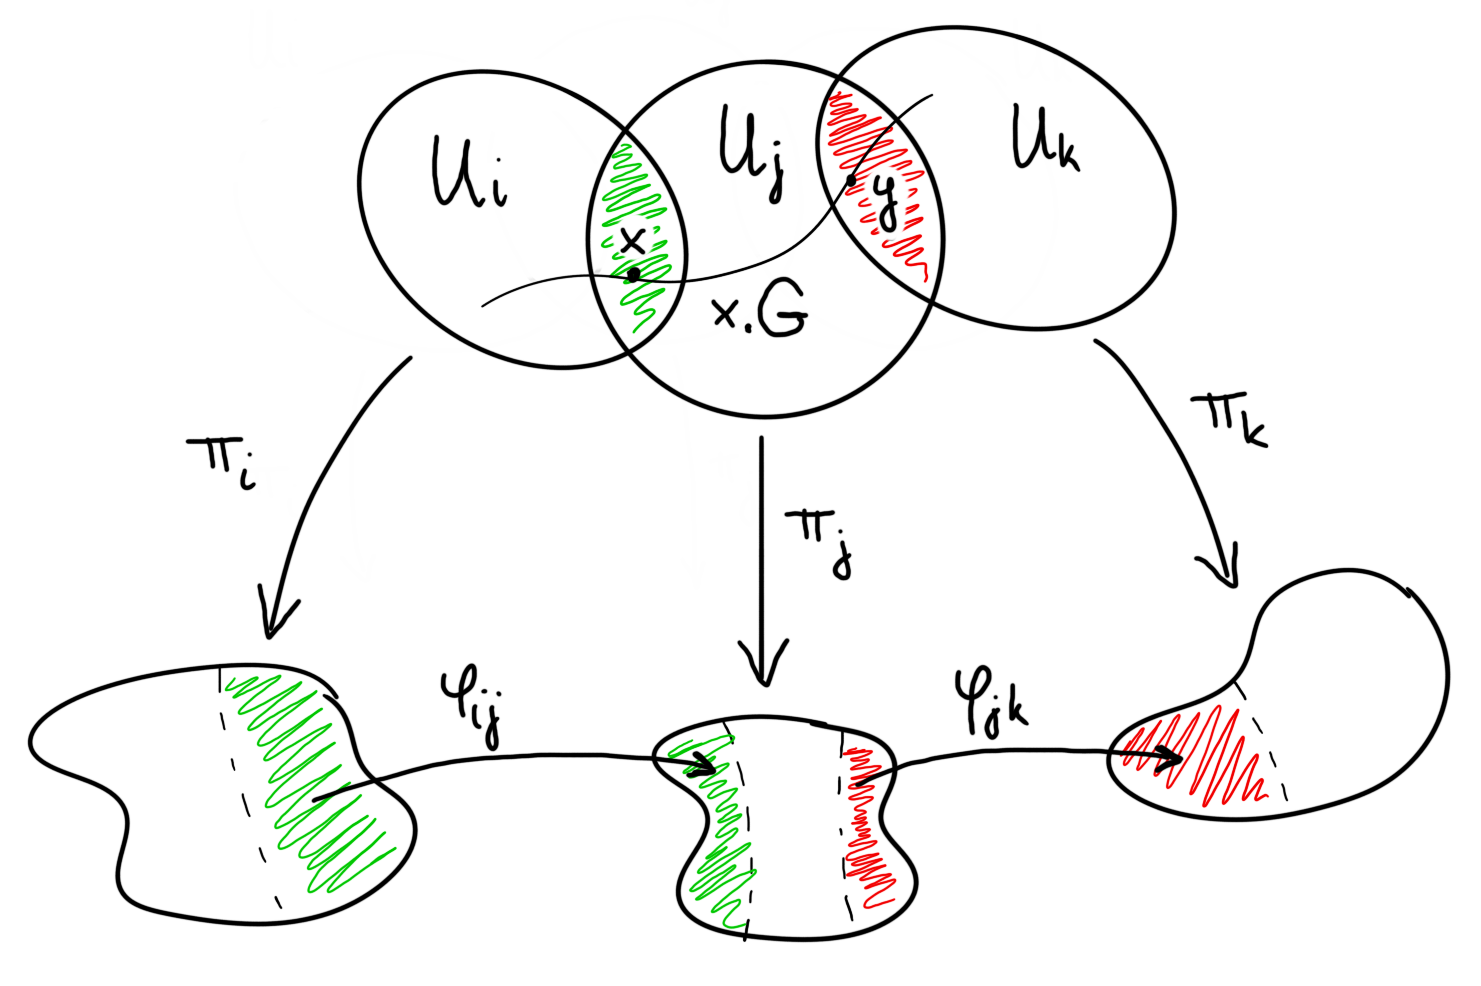
\includegraphics[scale=.9]{pictures/glueing.png}
    \end{figure}

    So in this case we do have $q_{j}(U_{i,j,k}) = q_{j}(U_{i,j}) \cap q_{j}(U_{j,k})$.
    And similarly $q_{i}(U_{i,j}) \cap q_{i}(U_{i,k}) = q_{i}(U_{i,j,k})$, so we need to show that $\varphi_{i,j}(q_{i}(U_{i,j,k})) = q_{j}(U_{i,j,k})$.
    But by construction we have $\varphi_{i,j} \circ q_{i,j} = q_{j,i}$, and this implies the desired equality.
    Hence $\varphi_{i,k}|_{q_{i}(U_{i,j,k})}$ and $\varphi_{j,k} \circ \varphi_{i,j}|_{q_{i}(U_{i,j,k})}$ are two isomorphisms between $q_{i}(U_{i,j,k})$ and $q_{k}(U_{i,k}) \cap q_{k}(U_{i,j}) = q_{k}(U_{i,j,k})$.
    But the corestriction of each $q_{i}$ to $q_{i}(U_{i,j,k})$ is also a geometric quotient of $U_{i,j,k}$ by $G$, so there exist unique isomorphisms $\psi_{i,k} \colon q_{i}(U_{i,j,k}) \cong q_{k}(U_{i,j,k})$ under $U_{i,j,k}$.
    In particular, since $\varphi_{i,k}|_{q_{i}(U_{i,j,k})}$ and $\varphi_{j,k} \circ \varphi_{i,j}|_{q_{i}(U_{i,j,k})}$ are two such isomorphisms, they must be equal, as we wanted to show.
    Hence the cocycle condition is satisfied and we may glue the $q_{i}$ together to obtain a $\mathbb{C}$-scheme morphism $q \colon X \to Z$ for some $\mathbb{C}$-scheme $Z$ obtained by glueing the $U_{i}/G$ together \cite[Exercise II.2.12]{har77}.
    Finally, since being a geometric quotient is local on the target, it suffices to show that this resulting morphism $q \colon X \to Z$ is a geometric quotient on an open cover of $Z$.
    But by construction $Z$ has an open cover $\{ V_{i} \}_{i \in I}$ in which each $V_{i}$ is identified with $U_{i}/G$ in such a way that the corresponding corestriction $q|_{q^{-1}(V_{i})} \colon q^{-1}(V_{i}) \to V_{i}$ is identified with the geometric quotient $q_{i} \colon U_{i} \to U_{i}/G$, so we are done.
  \end{proof}
\end{lm}

\begin{lm}\label{lm:avoidpoints}
  Let $X$ be a quasi-projective $\mathbb{C}$-scheme and let $x_{1},\ldots, x_{m} \in X$ be finitely many closed points.
  Then there exists an affine open subset $U \subseteq X$ such that $x_{i} \in U$ for all $i \in \{ 1, \ldots, m\}$.
  \begin{proof}
    We reproduce here the argument given in the notes that we are following most of the time, cited above.
    We regard $X$ as a locally closed subset of some $\mathbb{P}^{n}$.
    Then we look at its Zariski closure $\bar{X}$.
    If we find a hypersurface $H \subseteq \mathbb{P}^{n}$ which contains $\bar{X} \setminus X$ but not $x_{1}, \ldots, x_{m}$, then we are done, because $\mathbb{P}^{n} \setminus H$ is affine\footnote{If $H$ is a hyperplane, then $\mathbb{P}^{n} \setminus H \cong \mathbb{A}^{n}$.
    If $H$ is a hypersurface of degree $d$, then we may regard it as the intersection of a hyperplane with the image of $\mathbb{P}^{n}$ under the corresponding Veronese embedding, so the image of $\mathbb{P}^{n} \setminus H$ would be a closed subset inside the affine space given by the complement of this hyperplane, hence affine itself.} and $U := X \setminus H = \bar{X} \setminus H$ is closed inside an affine, hence affine itself.
    
    The main ingredient to find the hypersurface $H$ is the graded prime avoidance lemma \cite[\href{https://stacks.math.columbia.edu/tag/00JS}{Tag 00JS}]{stacks-project}.
    Let $\mathbb{C}[z_{0},\ldots,z_{n}]$ be the homogeneous coordinate ring of $\mathbb{P}^{n}$.
    If $\bar{X} = X$, we take $I$ to be $(z_{0}, \ldots, z_{n})$.
    Otherwise we take $I$ to be the homogeneous ideal of $\bar{X} \setminus X$.
    We take $\mathfrak{p}_{i}$ to be the maximal ideal corresponding to the point $x_{i}$ for each $i \in \{1, \ldots, m\}$.
    Let $i \in \{ 1, \ldots, m\}$.
    We have $(z_{0}, \ldots, z_{n}) \not\subset \mathfrak{p}_{i}$, because the maximal ideal $(z_{0}, \ldots, z_{n})$ does not correspond to any point in $\mathbb{P}^{n}$.
    And $x_{i} \not \in \bar{X} \setminus X$, because $x_{i} \in X$ by assumption.
    So in any case we have $I \not \subset \mathfrak{p}_{i}$.
    Hence we may apply graded prime avoidance to deduce the existence of a homogeneous polynomial of positive degree $f \in I$ which is not in any of the $\mathfrak{p}_{i}$, i.e.~such that $x_{i}$ is not in the hypersurface defined by $f$ for any $i \in \{1, \ldots, m\}$.
  \end{proof}
\end{lm}

\begin{thm}\label{thm:quotient}
  Let $\sigma \colon X \times G \to X$ be an action of a finite group on a quasi-projective $\mathbb{C}$-scheme.
  Then the geometric quotient $q \colon X \to X/G$ of $X$ by $G$ exists.
  The resulting $\mathbb{C}$-scheme $X/G$ is separated and of finite type over $\mathbb{C}$.
  Moreover, let $\mathbf{P}$ be any of the following properties:
  \begin{enumerate}[label=(\alph*)]
    \item irreducible,
    \item reduced,
    \item integral,
    \item normal,
    \item affine,
    \item projective.
  \end{enumerate}
  If $X$ has $\mathbf{P}$, then $X/G$ has $\mathbf{P}$.
  In particular, if $X$ is a (projective) variety, then $X/G$ is a (projective) variety.

  \begin{proof}
    We start by checking the existence of the geometric quotient with \Cref{lm:affinecover}.
    Since $X$ is quasi-projective over $\mathbb{C}$, it is also of finite type over $\mathbb{C}$, so it remains to find a $G$-invariant affine open cover of $X$.
    The orbit of every closed point $x \in X$ is contained in some affine open subset $U_{x}$ by \Cref{lm:avoidpoints}.
    It may be the case that $U_{x}$ is not yet $G$-invariant, but in any case the open neighborhood $\cap_{g \in G} U_{x}\cdot g$ of $x$ is $G$-invariant.
    Since $X$ is quasi-projective over $\mathbb{C}$, it is also separated, so the intersection of finitely many affine open subsets is again an affine open subset.
    Therefore we are able to find a $G$-invariant affine open neighborhood around each closed point of $X$, and by \Cref{lm:affinecover} the geometric quotient $q \colon X \to X/G$ of $X$ by $G$ exists.

    We show next separatedness of $X/G$ over $\mathbb{C}$.
    Note that $q \colon X \to X/G$ is finite and surjective, because we may check these properties on an open cover of the target and by construction of $X/G$ we may then assume that we are in the situation of \Cref{lm:finitesurjective}.
    We can then apply \cite[\href{https://stacks.math.columbia.edu/tag/09MQ}{Tag 09MQ}]{stacks-project} to deduce separatedness of $X/G$ over $\mathbb{C}$.

    The construction of $X/G$ combined with \Cref{lm:finitetype} shows that $X/G$ is locally of finite type over $\mathbb{C}$, and since $X$ is quasi-compact and $q$ is surjective, so is $X/G$.
    Hence $X/G$ is of finite type over $\mathbb{C}$.
    
    About the remaining properties $\mathbf{P}$ in the statement:
    \begin{enumerate}[label=(\alph*)]
      \item Since $q$ is surjective, so $X/G$ is irreducible as soon as $X$ is.
      \item Reducedness can be checked locally on $X/G$, so by construction of $X/G$ we may assume that we are in the situation of \Cref{cor:affinequotient}.
        But the corresponding ring morphism $A^{G} \to A$ is just the inclusion, so $A^{G}$ is reduced as soon as $A$ is reduced.
      \item The same argument as for reducedness applies, or one can also argue using that being integral is equivalent to being reduced and irreducible.
      \item Normality can again be checked locally on $X/G$, so we may assume that we are in the situation of \Cref{cor:affinequotient}.
        We need to show that $A^{G}$ is an integrally closed domain if $A$ is an integrally closed domain.
        For this we use compatibility of taking $G$-invariant subrings with localization \cite[Exercise 5.12]{am69}.
        Let $f \in (A^{G})_{(0)} = (A_{(0)})^{G}$ be a $G$-invariant element in the field of fractions of $A^{G}$, which is the subfield of $G$-invariant elements of the field of fractions of $A$.
        Suppose that $f$ is integral over $A^{G}$, i.e.~supposet that $f$ is the root of some monic polynomial with coefficients in $A^{G}$.
        We regard this monic polynomial as a monic polynomial with coefficients in $A$, which shows that $f$ is an element of $A_{(0)}$ which is integral over $A$.
        Since $A$ is integrally closed, this element of $A_{(0)}$ must already be in $A$.
        And it is $G$-invariant as well, so $f \in A^{G}$.
      \item If $X$ is affine, then we may apply \Cref{cor:affinequotient} directly to conclude that $X/G$ is affine as well.
      \item Properness of $X/G$ over $\mathbb{C}$ follows from the things that we have shown already, since the image of a proper scheme in a separated scheme of finite type is proper \cite[\href{https://stacks.math.columbia.edu/tag/03GN}{Tag 03GN}]{stacks-project}.
        An argument for the projectivity, which in fact shows that $X/G$ is quasi-projective as soon as $X$ is, can be found in \cite[Proposition IV.1.5]{knu71}.
        Projectivity would also follow from the more general GIT machinery.
    \end{enumerate}
  \end{proof}
\end{thm}

\bibliographystyle{alpha}
\bibliography{main}
\vfill

\end{document}
